% A clean IEEEtran conference paper with page numbers, a raster figure, a plot over the text width, tables, an
% algorithm, a listing with line numbers, footnotes, and long URLs, each placed as the template intends.
\pdftrailerid{}
\pdfinfoomitdate=1
\pdfsuppressptexinfo=-1
\documentclass[10pt,conference,letterpaper]{IEEEtran}
\usepackage{amsmath}
\usepackage{graphicx}
\usepackage{booktabs}
\usepackage{multirow}
\usepackage{xcolor}
\usepackage{listings}
\usepackage{algorithm}
\usepackage{algorithmic}
\usepackage{pgfplots}
\pgfplotsset{compat=1.18}
\usepackage{lipsum}
\usepackage{url}
\usepackage[hidelinks]{hyperref}
\lstset{basicstyle=\ttfamily\footnotesize, frame=single, numbers=left, numberstyle=\tiny,
  xleftmargin=2em, framexleftmargin=1.5em, breaklines=true, columns=fullflexible}
\begin{document}
\title{Ranking Flaky Test Failures with\\Build Histories and Change Distance}
\author{\IEEEauthorblockN{Anonymous Author(s)}}
\maketitle
\thispagestyle{plain}
\pagestyle{plain}

\begin{abstract}
Flaky tests pass and fail on the same code. This paper ranks the failures of a build by the
chance that each failure is flaky. On 4,210 failures of ten projects, the ranking places the
flaky failure first in 71\% of the builds. The data and scripts are available at
\url{https://anonymous.4open.science/r/flaky-ranking-replication-package-2027}.
\end{abstract}

\begin{IEEEkeywords}
flaky tests, regression testing, continuous integration
\end{IEEEkeywords}

\section{Introduction}
\lipsum[1-2]
The study builds on the public logs of the projects, such as
\url{https://github.com/apache/commons-lang/actions/workflows/maven.yml?query=branch%3Amaster+event%3Apush}
and the issue tracker at
\url{https://issues.apache.org/jira/projects/LANG/issues/LANG-1700?filter=allopenissues}.\footnote{The
build logs come from \url{https://api.github.com/repos/apache/commons-lang/actions/runs?per_page=100&page=1}.}

\section{Background}
\lipsum[4]
Fig.~\ref{fig:raster} shows a build page.\footnote{A second footnote with a long address,
\url{https://docs.github.com/en/actions/using-workflows/events-that-trigger-workflows\#workflow_run}.}

\begin{figure}[t]
\centering
\includegraphics[width=\columnwidth]{example-image-16x9.png}
\caption{A build page as a raster image of the full column width.}
\label{fig:raster}
\end{figure}

\section{Approach}
\lipsum[6]
Algorithm~\ref{alg:rank} gives the ranking, and Listing~\ref{lst:test} a flaky test.

\begin{algorithm}[t]
\caption{Rank the failures of one build}
\label{alg:rank}
\begin{algorithmic}[1]
\REQUIRE failures $F$, history $H$, changed files $C$
\FORALL{$f \in F$}
\STATE $s_f \gets \alpha \cdot \mathrm{rerun}(f, H) + \beta \cdot \mathrm{distance}(f, C)$
\ENDFOR
\RETURN $F$ sorted by $s_f$ in descending order
\end{algorithmic}
\end{algorithm}

\begin{lstlisting}[language=Java, caption={A test that depends on the order of the suite.}, label={lst:test}]
@Test
public void readsSharedCache() {
    assertEquals(0, SharedCache.getInstance().size());
    SharedCache.getInstance().put("key", computeExpensiveValueFromTheNetwork("https://example.org"));
}
\end{lstlisting}

\lipsum[7]
\begin{equation}
\begin{split}
s_f ={}& \alpha \cdot \frac{\lvert \{ b \in H : f \in \mathrm{passed}(b) \} \rvert}{\lvert H \rvert}\\
  &+ \beta \cdot \frac{1}{1 + \mathrm{distance}(f, C)}
\end{split}
\end{equation}

\begin{figure*}[t]
\centering
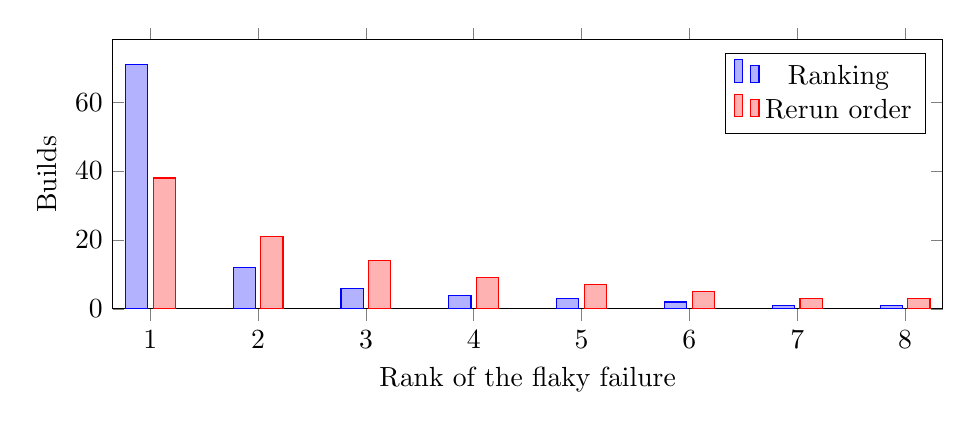
\begin{tikzpicture}
\begin{axis}[width=\textwidth, height=5cm, xlabel={Rank of the flaky failure},
  ylabel={Builds}, ybar, bar width=8pt, xtick=data, ymin=0, enlarge x limits=0.05,
  legend style={at={(0.98,0.95)}, anchor=north east}]
\addplot coordinates {(1,71) (2,12) (3,6) (4,4) (5,3) (6,2) (7,1) (8,1)};
\addplot coordinates {(1,38) (2,21) (3,14) (4,9) (5,7) (6,5) (7,3) (8,3)};
\legend{Ranking, Rerun order}
\end{axis}
\end{tikzpicture}
\caption{Rank of the flaky failure in each build, over the full text width.}
\label{fig:ranks}
\end{figure*}

\section{Evaluation}
\lipsum[8]
Table~\ref{tab:projects} lists the projects, and Table~\ref{tab:ranks} the ranks.

\begin{table}[t]
\caption{Projects and failures}
\label{tab:projects}
\centering
\resizebox{\columnwidth}{!}{%
\begin{tabular}{lrrrr}
\toprule
Project & Tests & Builds & Failures & Flaky failures \\
\midrule
commons-lang & 4,120 & 1,210 & 512 & 61 \\
guava & 18,330 & 2,004 & 1,120 & 133 \\
jsoup & 1,020 & 803 & 214 & 30 \\
\multirow{2}{*}{spring-boot} & \multirow{2}{*}{12,880} & 1,540 & 902 & 140 \\
 & & 210 & 77 & 9 \\
\midrule
Total & 36,350 & 5,767 & 2,825 & 373 \\
\bottomrule
\end{tabular}}
\end{table}

\lipsum[9-10]

\begin{table*}[t]
\caption{Rank of the flaky failure per project and method}
\label{tab:ranks}
\centering
\begin{tabular*}{\textwidth}{@{\extracolsep{\fill}}lrrrrrrrrrr@{}}
\toprule
Method & lang & guava & jsoup & spring & netty & kafka & flink & hadoop & hbase & Total \\
\midrule
Ranking & 61 & 133 & 30 & 140 & 88 & 120 & 95 & 160 & 110 & 937 \\
Rerun order & 33 & 70 & 16 & 77 & 41 & 64 & 52 & 85 & 62 & 500 \\
Random & 12 & 25 & 5 & 30 & 18 & 22 & 20 & 31 & 24 & 187 \\
\bottomrule
\end{tabular*}
\end{table*}

\lipsum[11-13]

\section{Conclusion}
\lipsum[15]

\begin{thebibliography}{9}
\bibitem{luo} Q. Luo, F. Hariri, L. Eloussi, and D. Marinov, ``An empirical analysis of flaky
tests,'' in \emph{Proc. FSE}, 2014, pp. 643--653.
\bibitem{lam} W. Lam, R. Oei, A. Shi, D. Marinov, and T. Xie, ``iDFlakies: A framework for
detecting and partially classifying flaky tests,'' in \emph{Proc. ICST}, 2019, pp. 312--322.
\bibitem{data} Apache Software Foundation, ``Build logs of the commons-lang project,'' 2026.
[Online]. Available: \url{https://github.com/apache/commons-lang/actions/runs/1234567890/job/9876543210}
\bibitem{gh} GitHub, ``Events that trigger workflows,'' 2026. [Online]. Available:
\url{https://docs.github.com/en/actions/writing-workflows/choosing-when-your-workflow-runs/events-that-trigger-workflows}
\end{thebibliography}
\end{document}
